\chapter{Introduction}
\section{Installation}
\clearpage
\section{Overview}
\begin{center}
    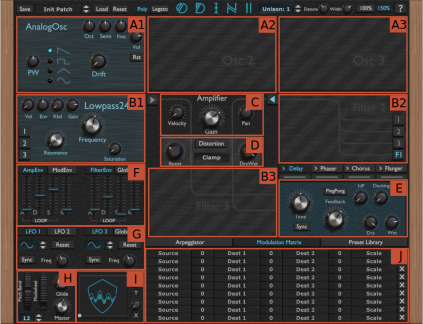
\includegraphics[width=\textwidth]{graphics/overview.png}
\end{center}

\begin{itemize}
    \item \fat{A}: The three oscillator slots. See Chapter \ref{oscillators}.
    \item \fat{B}: The three filter slots. See Chapter \ref{filters}.
    \item \fat{C}: The amplifier module. See Chapter \ref{amplifier}.
    \item \fat{D}: The distortion module. See Chapter \ref{distortion}.
    \item \fat{E}: The FX section: See Chapter \ref{FX}.
    \item \fat{F}: The four ADSR Envelopes.
    \item \fat{G}: The four Low Frequency Oscillators (LFOs).
    \item \fat{H}: The global controls
    \item \fat{I}: The XY-pad section.
    \item \fat{J}: The Modulation Matrix. This space can also be occupied by the arpeggiator and preset browser.
\end{itemize}
\section{Saving and Loading Presets}
\section{Routing}
\label{routing}
